\documentclass{standalone}
\usepackage{tikz}
\usetikzlibrary{calc}
\begin{document}
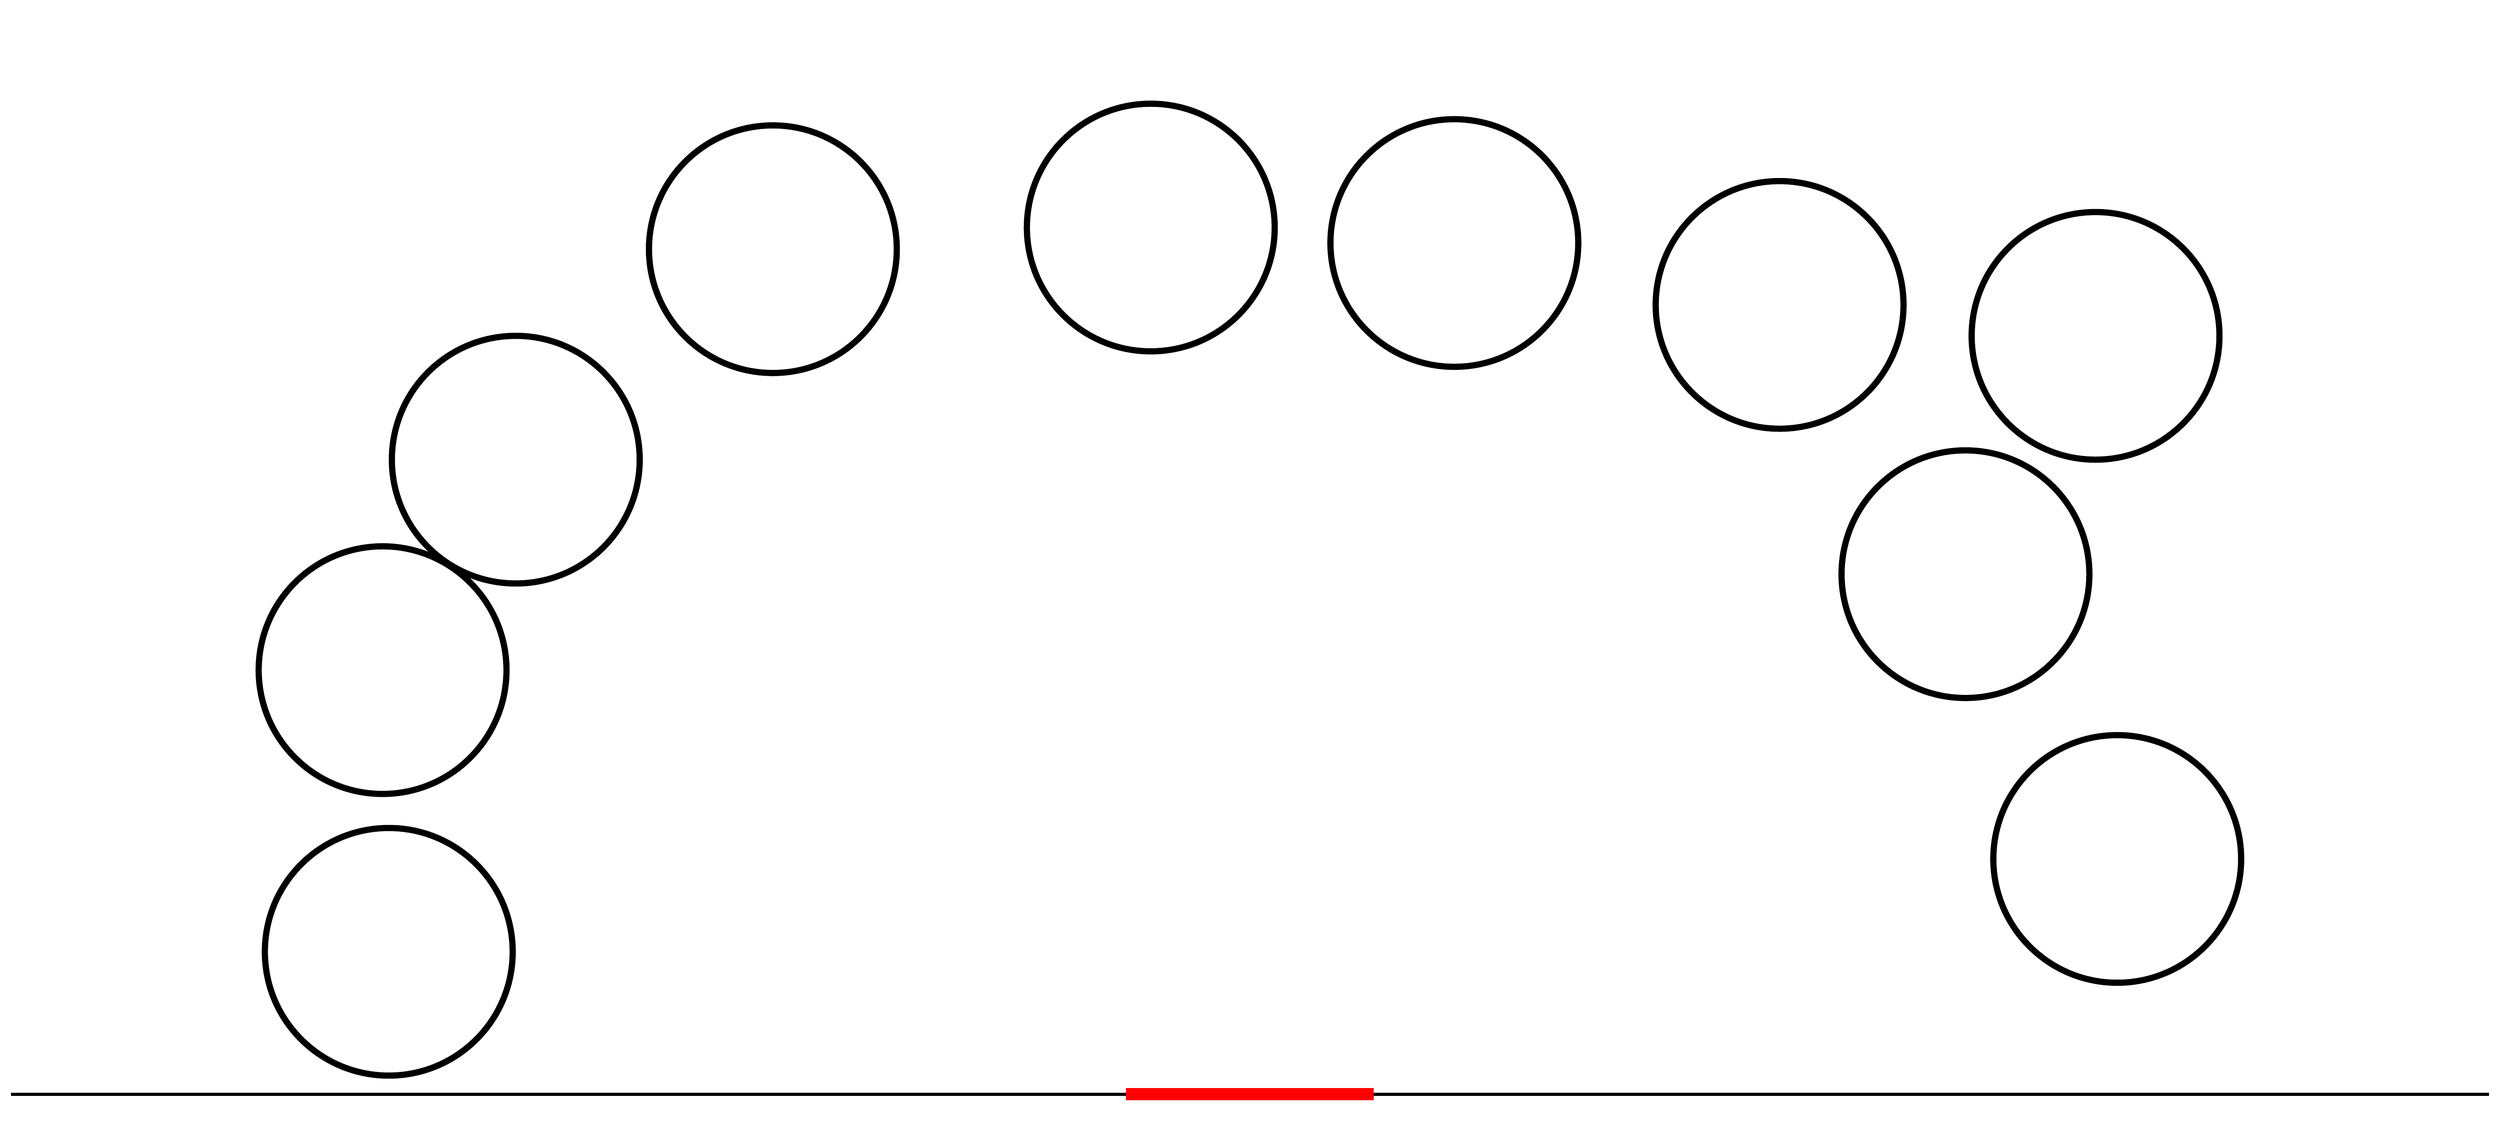
\begin{tikzpicture}[x=0.125cm, y=0.125cm, scale=0.8]

\useasboundingbox (-400,-10) rectangle (400,350);

\draw[line width=1mm] (-400,0) -- (400,0);
\draw[line width=4mm, red] (-40,0) -- (40,0);
\draw[line width=2mm] (273,245) circle (5cm);
\draw[line width=2mm] (171,255) circle (5cm);
\draw[line width=2mm] (-154,273) circle (5cm);
\draw[line width=2mm] (-237,205) circle (5cm);
\draw[line width=2mm] (-280,137) circle (5cm);
\draw[line width=2mm] (280,76) circle (5cm);
\draw[line width=2mm] (231,168) circle (5cm);
\draw[line width=2mm] (-32,280) circle (5cm);
\draw[line width=2mm] (66,275) circle (5cm);
\draw[line width=2mm] (-278,46) circle (5cm);

\end{tikzpicture}
\end{document}
